\documentclass[11pt,a4paper]{article}
\usepackage[margin=2cm]{geometry}
\usepackage{graphicx}
\graphicspath{{../results/images/}}
\usepackage{booktabs}
\usepackage{float}
\usepackage{caption}
\setlength{\parindent}{0pt}
\pagestyle{empty}

\begin{document}

\begin{center}
{\Large\bfseries Flow Simulation Results -- Paddy-Store Sensor Node}\\[4pt]
SOLIDWORKS Flow Simulation 2024 \quad|\quad Room air 32\,\textdegree C, 70\,\% RH, still air
\end{center}

\section*{Defined conditions}
\begin{table}[H]
\centering
\begin{tabular}{l l}
\toprule
Parameter & Value \\
\midrule
Analysis type & External, steady state \\
Fluid & Humid air (laminar and turbulent) \\
Room air temperature & 32\,\textdegree C \\
Relative humidity & 70\,\% \\
Pressure & 101.325\,kPa \\
Air velocity & 0\,m/s (still air, natural convection) \\
Gravity & 9.81\,m/s$^2$, device hanging, sensor holder below box \\
Radiation & On, surroundings 32\,\textdegree C, no solar \\
Surface emissivity (printed parts) & 0.9 \\
Heat conduction in solids & On \\
\midrule
ESP-12F heat & 0.50\,W \\
8 resistors heat & 0.40\,W \\
LDO regulator (SOT-223) heat & 0.25\,W \\
Q1 (TO-220) heat & 0.20\,W \\
Total PCB heat & 1.35\,W (continuous) \\
RH/T sensor board heat & 0\,W \\
\midrule
Enclosure material & PLA+ (white) \\
\quad Density & 1230\,kg/m$^3$ \\
\quad Thermal conductivity & 0.15\,W/m$\cdot$K \\
\quad Specific heat & 1800\,J/kg$\cdot$K \\
\quad Softening limit & 55\,\textdegree C \\
PCB material & FR4 \\
\midrule
Mesh & Level 5, minimum gap 1.5\,mm, 3\,158\,364 cells \\
Convergence & 382 iterations, all goals converged \\
\bottomrule
\end{tabular}
\end{table}

\section*{Main results}
\begin{table}[H]
\centering
\begin{tabular}{l c c c}
\toprule
Result & Value & Room air & Difference \\
\midrule
Sensor chip temperature & 32.12\,\textdegree C & 32.00\,\textdegree C & +0.12\,\textdegree C \\
Air temperature in sensor holder & 32.08 -- 32.27\,\textdegree C & 32.00\,\textdegree C & +0.08 to +0.27\,\textdegree C \\
Relative humidity in sensor holder & 68.9 -- 69.7\,\% & 70.0\,\% & $-$0.3 to $-$1.1\,\% \\
Air inside box (near PCB) & 41.52\,\textdegree C, 42.0\,\% RH & -- & +9.52\,\textdegree C \\
Warm air above box & 34.95 -- 35.65\,\textdegree C & 32.00\,\textdegree C & +2.95 to +3.65\,\textdegree C \\
Hottest PLA+ part & $\approx$50.4\,\textdegree C & limit 55\,\textdegree C & 4.6\,\textdegree C margin \\
ESP-12F hottest point & 82.5\,\textdegree C & -- & -- \\
\bottomrule
\end{tabular}
\end{table}

\section*{Probe points}
\begin{table}[H]
\centering
\small
\begin{tabular}{r l r r r r}
\toprule
\# & Location & Temp (\textdegree C) & Rise (\textdegree C) & RH (\%) & Speed (m/s) \\
\midrule
1  & Sensor chip surface                     & 32.12 & +0.12 & --   & --     \\
2  & Sensor holder, centre upper             & 32.27 & +0.27 & 68.9 & 0.0007 \\
3  & Sensor holder, centre lower             & 32.15 & +0.15 & 69.4 & 0.0005 \\
4  & Sensor holder, right                    & 32.09 & +0.09 & 69.6 & 0.012  \\
5  & Sensor holder, left                     & 32.08 & +0.08 & 69.7 & 0.012  \\
6  & Sensor holder, front                    & 32.08 & +0.08 & 69.7 & 0.012  \\
7  & Sensor holder, back                     & 32.09 & +0.09 & 69.7 & 0.014  \\
8  & Sensor holder, outer edge               & 32.01 & +0.01 & 70.0 & 0.004  \\
9  & Neck between box and holder             & 32.23 & +0.23 & 69.1 & 0.048  \\
10 & 35\,mm below holder                     & 32.01 & +0.01 & 70.0 & 0.001  \\
11 & 75\,mm below holder                     & 32.00 & 0.00  & 70.0 & 0.001  \\
12 & Room air beside box                     & 32.03 & +0.03 & 69.9 & 0.006  \\
13 & Inside box near PCB                     & 41.52 & +9.52 & 42.0 & 0.044  \\
14 & Inside box near neck                    & 33.12 & +1.12 & 65.7 & 0.004  \\
15 & 20\,mm above box                        & 35.65 & +3.65 & 57.3 & 0.075  \\
16 & 80\,mm above box                        & 35.58 & +3.58 & 57.4 & 0.143  \\
17 & 180\,mm above box                       & 34.95 & +2.95 & 59.4 & 0.186  \\
\bottomrule
\end{tabular}
\end{table}

\section*{Heat balance}
\begin{table}[H]
\centering
\begin{tabular}{l r r}
\toprule
Item & Power & Share \\
\midrule
Total PCB heat & 1.35\,W & 100\,\% \\
Convection to air & 0.70\,W & 52\,\% \\
Radiation & 0.65\,W & 48\,\% \\
\bottomrule
\end{tabular}
\end{table}

\section*{Sensor position comparison}
\begin{table}[H]
\centering
\begin{tabular}{l c c}
\toprule
Sensor position & Sensor temperature & Sensor RH \\
\midrule
Above box & $\approx$49\,\textdegree C & 26 -- 31\,\% \\
Below box (final) & 32.12\,\textdegree C & 68.9 -- 69.7\,\% \\
\bottomrule
\end{tabular}
\end{table}

\section*{Result plots}
\begin{figure}[H]
\centering
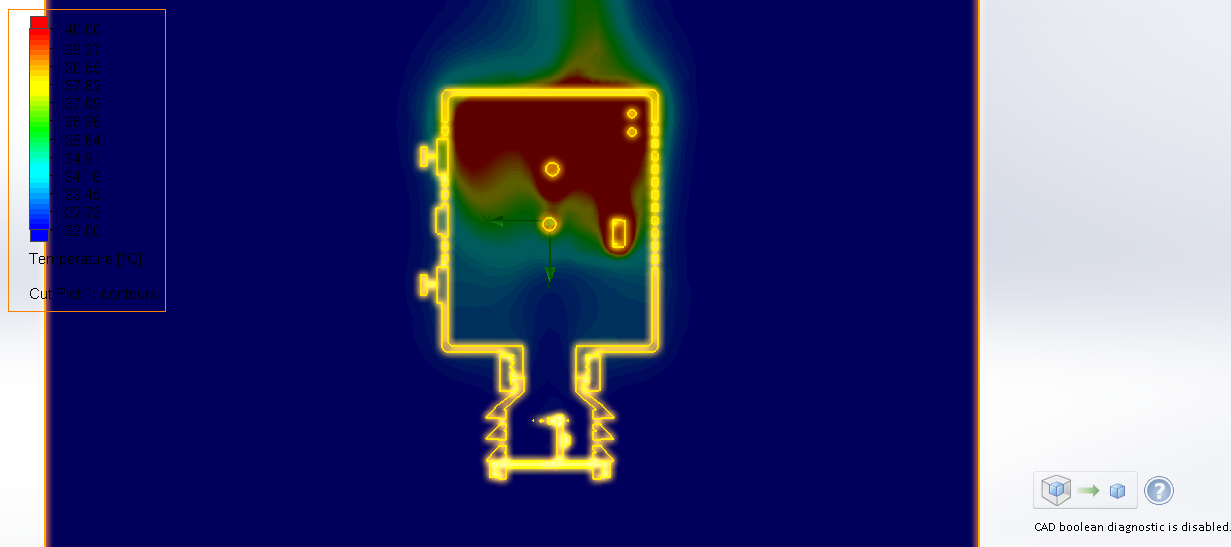
\includegraphics[width=\linewidth]{01 Temperature section front.png}
\caption*{Temperature section}
\end{figure}

\begin{figure}[H]
\centering
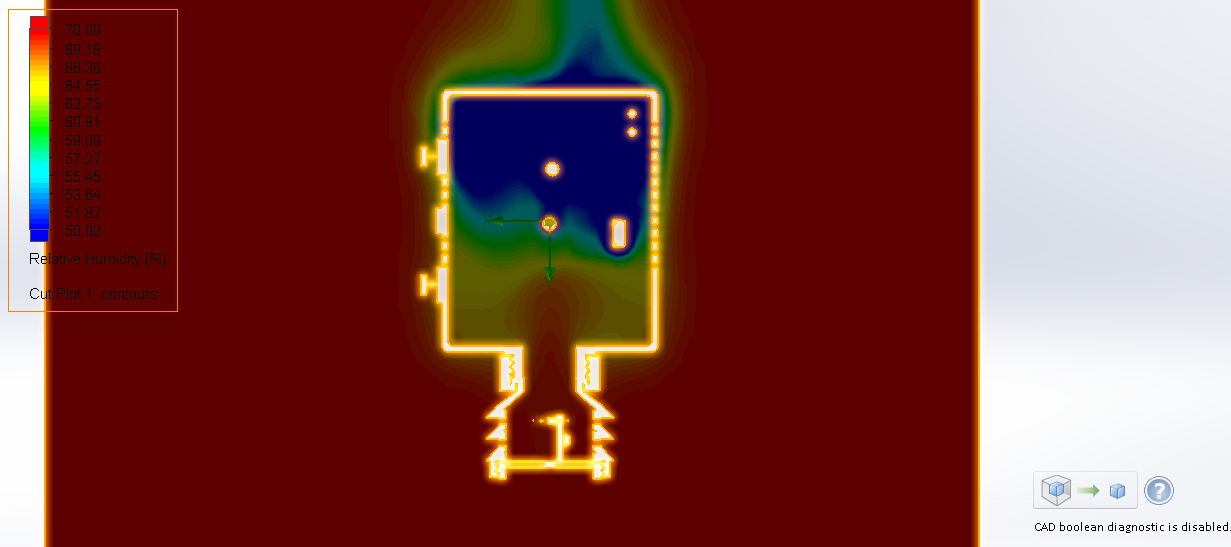
\includegraphics[width=\linewidth]{02 Relative humidity section front.png}
\caption*{Relative humidity section}
\end{figure}

\begin{figure}[H]
\centering
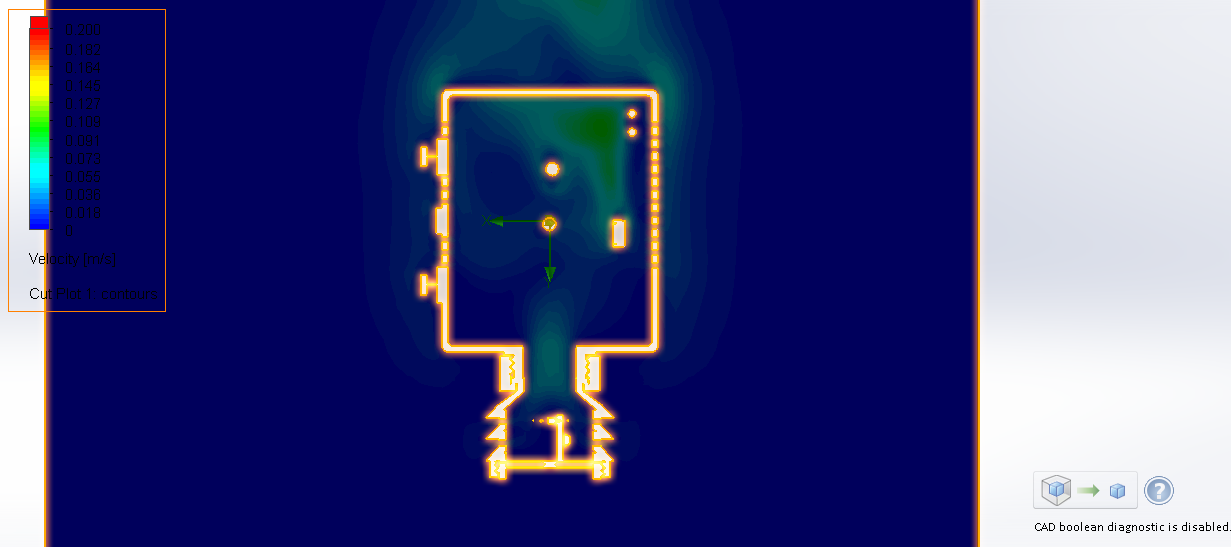
\includegraphics[width=\linewidth]{03 Air speed section front.png}
\caption*{Air speed section}
\end{figure}

\begin{figure}[H]
\centering
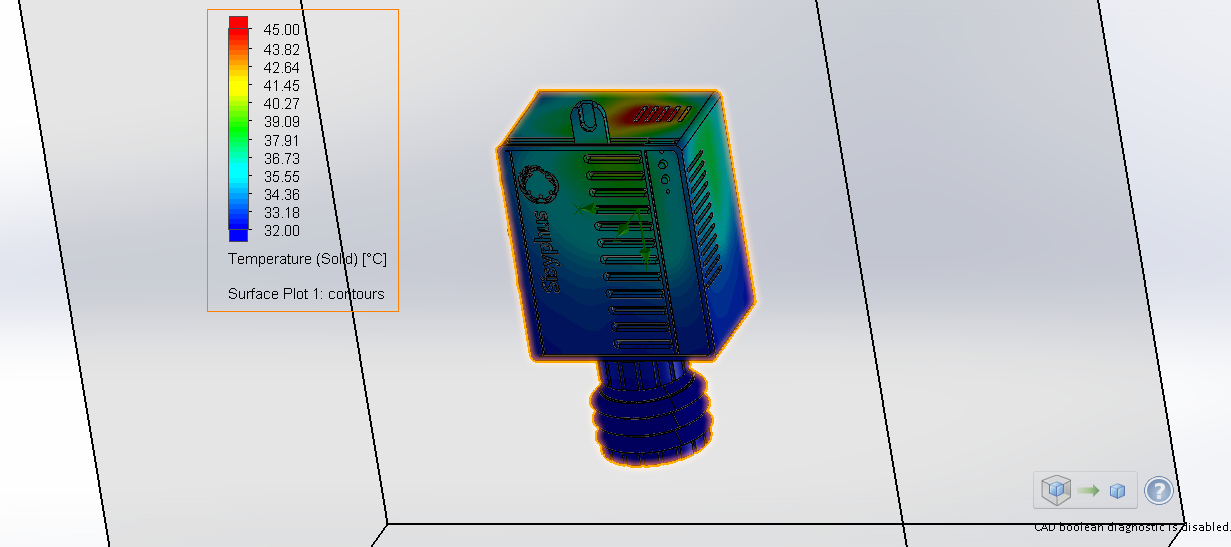
\includegraphics[width=\linewidth]{04 Surface temperature 3D.png}
\caption*{Surface temperature}
\end{figure}

\end{document}
